\documentclass[11pt]{article}
\usepackage[letterpaper,margin=0.88in]{geometry}
\usepackage{amsmath,amssymb,amsthm,booktabs,tabularx,microtype,hyperref,tikz}
\usetikzlibrary{arrows.meta,positioning}
\hypersetup{colorlinks=true,linkcolor=black,citecolor=black,urlcolor=black}
\newtheorem{theorem}{Theorem}[section]
\newtheorem{proposition}[theorem]{Proposition}
\newtheorem{corollary}[theorem]{Corollary}
\newtheorem{definition}[theorem]{Definition}
\newtheorem{example}[theorem]{Example}
\theoremstyle{remark}\newtheorem{remark}[theorem]{Remark}
\newcommand{\cl}{\operatorname{cl}}
\newcommand{\Opt}{\operatorname{OPT}}
\newcommand{\cU}{\mathcal U}
\newcommand{\cP}{\mathcal P}
\newcommand{\cO}{\mathcal O}
\newcommand{\hit}{\operatorname{Tr}}
\title{\textbf{The Geometry of Mathematical Obstruction}\\[4pt]\large Proof--Obstruction Duality, Certified Deductive Navigation,\\and MAPQUEST in the 24th Century}
\author{Research direction: Brian Tenneson\\Mathematical drafting and analysis: ChatGPT (Picard research protocol)}
\date{24 November 2026 \quad | \quad Research edition 001v2 (Atlas audit)}
\begin{document}
\maketitle
\begin{abstract}
A proof describes a sufficient collection of inference instances; an obstruction describes a condition that every successful collection must overcome. We develop this dual perspective for finite monotone deductive hypergraphs, where shared lemmas are charged once. Cut crossing, blocker duality, and a cut-based integer program recover established shortest-hyperpath and transversal mathematics. We use these foundations to develop a certificate-oriented approach to deductive navigation: rational cut prices give replayable lower bounds, surviving cuts transport information as verified knowledge grows, and an explicit forward relaxation permits lower bounds to transfer from a finite abstraction to a larger proof system. We prove a finite repair-cover criterion for independently composable edge additions and distinguish it from arbitrary operational revisions. An exhaustive small-model check accompanies the paper. The concluding sections specialize the mathematics to the MAPQUEST trilogy and then to a sovereign game, the ``24th century.'' The work is a mathematical research proposal with manuscript-level proofs, not an implemented theorem prover or a claim of speedup.
\end{abstract}
\noindent\textbf{Scope and provenance.} Sections 1--7 are independent of MAPQUEST and sovereign games. Sections 8--9 apply the results without modifying the three supplied source manuscripts. Known cut and blocker results are identified as such; the certificate transport and revision interfaces are developed here as research constructions, without a priority claim. The final target and its verifier are not changed by the proposed applications.\\
\noindent\textbf{Keywords:} deductive hypergraph; obstruction; proof DAG; weighted cut; certificate; automated theorem proving; sovereign revision.
\par\medskip\noindent\textbf{Reading map.} Sections 1--3 establish the deductive geometry and duality; Sections 4--7 develop cost certificates, transport, complexity and discovery. Sections 8--9 specialize to MAPQUEST and sovereign revision; Section 10 collects open obligations.
\newpage
\section{A finite deductive landscape}
Let $X$ be a finite set of formula identifiers (including any necessary context tags), $B\subseteq X$ an initial set of established formulas, $T\in X$ a target, and $E$ a finite set of individually identified inference instances. An instance $e$ consists of its premise set $P_e\subseteq X$, its single conclusion $q_e\in X$, and a rational cost $c_e\geq0$. Distinct instances may have identical premise and conclusion sets. Any ordered premise list, substitution, side condition or proof context needed for an actual certificate belongs to the instance's separate witness record. A zero-premise instance is allowed. In the abstract model all instances have fixed legality once their premises are present. Context-sensitive, consumable, or nonmonotone systems require a richer state model before the following results can be used.

For $A\subseteq E$, define $\cl_A(B)$ by starting from $B$ and repeatedly adjoining $q_e$ whenever $e\in A$ and $P_e$ is contained in the current set. The process terminates because $X$ is finite. It computes the least $A$-closed superset of $B$. A derivation is a finite list of instances in which each premise is in $B$ or is an earlier conclusion. Thus $T\in\cl_A(B)$ if and only if $A$ contains a derivation of $T$. The empty derivation is valid when $T\in B$.

\begin{definition}[Additive proof cost]
The cost of a derivation is the sum of the costs of its executed inference occurrences. Define
\[
J_E(B,T)=\min\left\{\sum_{e\in A}c_e:A\subseteq E,\ T\in\cl_A(B)\right\},
\]
with the minimum of the empty feasible family interpreted as $+\infty$.
\end{definition}
Every derivation determines a feasible support of cost no greater than its occurrence cost. Conversely, closure produces a derivation from each feasible support using an instance at most once. Hence $J_E$ is the exact minimum additive derivation cost. This identification relies on reusable knowledge and nonnegative, fixed costs. It does not measure how long it takes to discover the derivation or check the complete certificate. Every operational implementation must account for those costs separately.

\paragraph{Three views of discovery.} Forward closure identifies what can be derived. Backward search proposes possible dependencies of the target. An obstruction asks what every possible successful support must accomplish. The third view provides constraints, not automatically a preferred proof. Its value lies in the interaction with the first two.

\section{Proof cuts and necessary crossing}
\begin{definition}[Target cut]
For $T\notin B$, a target cut is a set $U\subseteq X\setminus B$ containing $T$. Let $\cU(B,T)$ be the family of these sets. Its crossing instances are
\[
\delta_E(U)=\{e\in E:q_e\in U,\ P_e\cap U=\varnothing\}.
\]
The condition on the entire premise set is essential; an inference with even one unavailable premise inside $U$ cannot introduce the first formula of $U$.
\end{definition}
\begin{theorem}[Cut characterization]\label{thm:cut}
For every $A\subseteq E$,
\[
T\in\cl_A(B)\quad\Longleftrightarrow\quad
A\cap\delta_E(U)\ne\varnothing\quad\text{for every }U\in\cU(B,T).
\]
\end{theorem}
\begin{proof}
If a derivation succeeds, its first conclusion in $U$ is obtained by an instance all of whose premises are outside $U$. It therefore crosses $U$. Conversely, if the closure $R=\cl_A(B)$ does not contain $T$, let $U=X\setminus R$. It is a target cut, and an $A$-instance crossing it would derive a new formula from premises in $R$, contrary to closure. If $T\in B$, the cut family is empty and both sides hold.
\end{proof}
\begin{figure}[ht]
\centering
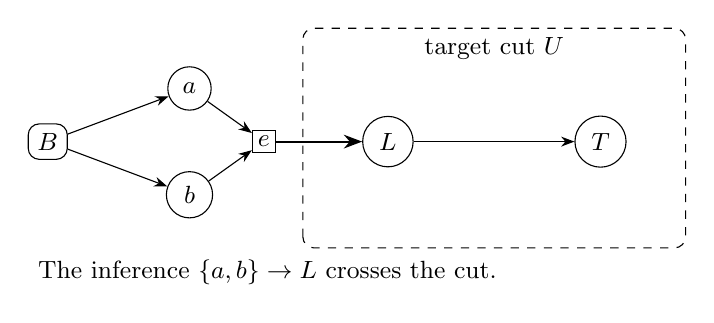
\begin{tikzpicture}[>=Stealth, every node/.style={font=\small}, scale=0.9]
\draw[dashed,rounded corners] (3.6,-1.5) rectangle (9,1.6);
\node at (6.3,1.32) {target cut $U$};
\node[draw,rounded corners] (b) at (0,0) {$B$};
\node[draw,circle] (a) at (2,0.75) {$a$};
\node[draw,circle] (d) at (2,-0.75) {$b$};
\node[draw,rectangle,inner sep=2pt] (e) at (3.05,0) {$e$};
\node[draw,circle] (l) at (4.8,0) {$L$};
\node[draw,circle] (t) at (7.8,0) {$T$};
\draw[->] (b)--(a); \draw[->] (b)--(d); \draw[->] (a)--(e); \draw[->] (d)--(e); \draw[->,thick] (e)--(l); \draw[->] (l)--(t);
\node at (3.1,-1.85) {The inference $\{a,b\}\to L$ crosses the cut.};
\end{tikzpicture}
\caption{A hyperedge crosses only when all its premises lie outside the cut. The illustration is schematic; it does not assert uniqueness of a crossing.}
\end{figure}
\begin{corollary}[Negative certificate]
A cut with $\delta_E(U)=\varnothing$ certifies that no derivation exists in the specified catalogue. If $T$ is not reachable, $X\setminus\cl_E(B)$ supplies such a cut.
\end{corollary}
Direct table checking of this certificate inspects every instance of the declared complete catalogue; a sound symbolic summary of the same complete catalogue may replace enumeration. It is not a certificate of underivability in a larger formal system whose instances have not been accounted for. The cut characterization is a single-head version of established directed-hypergraph reachability and shortest-hyperpath mathematics \cite{survey,krieger}.

\section{Proof--obstruction duality}
\begin{definition}
Let $\cP$ be the inclusion-minimal subsets of $E$ that derive $T$ from $B$. Let $\cO$ be the inclusion-minimal subsets $O\subseteq E$ for which $T\notin\cl_{E\setminus O}(B)$. For a family $\mathcal F$, write $\hit(\mathcal F)$ for its family of inclusion-minimal hitting sets.
\end{definition}
\begin{theorem}[Blocker duality and cut identification]\label{thm:dual}
\[
\cO=\hit(\cP),\qquad \cP=\hit(\cO),\qquad
\cO=\min_{\subseteq}\{\delta_E(U):U\in\cU(B,T)\}.
\]
\end{theorem}
\begin{proof}
Removal of $O$ prevents success exactly when $O$ intersects every minimal successful support. Taking minimal sets proves the first identity. A set $A$ is successful exactly when it hits every minimal removal obstruction: if not successful, $E\setminus A$ contains such an obstruction; if it misses one, it is contained in the remaining unsuccessful catalogue. Minimality proves the second identity. Removing all crossing instances of any cut prevents success by Theorem~\ref{thm:cut}. Conversely, for any removal obstruction $O$, closure under $E\setminus O$ gives a cut whose crossings are contained in $O$. Taking minimal elements yields the third identity.
\end{proof}
This includes the degenerate cases: an initially established target has $\cP=\{\varnothing\}$ and $\cO=\varnothing$; a target unreachable even with all of $E$ has $\cP=\varnothing$ and $\cO=\{\varnothing\}$. No hitting set exists for a family containing the empty set, and the unique minimal hitting set of an empty family is empty.

The first two identities are classical hypergraph transversal duality, not a new combinatorial theorem \cite{eiter}. The deductive interpretation is useful because proof checking and closure provide complementary oracles. It does not imply that all minimal proofs or obstructions can be listed efficiently. For example, $m$ independent choices between two parallel instances along a chain yield $2^m$ minimal proofs with only $2m$ instances. Conversely, $m$ disjoint two-edge paths from a seed to a target have $2^m$ minimal removal obstructions.

\section{Cost certificates and obstruction-directed optimization}
\begin{theorem}[Cut optimization]\label{thm:ip}
The following integer program has optimum $J_E(B,T)$, with infeasibility interpreted as $+\infty$:
\begin{align}
\min\quad&\sum_{e\in E}c_e x_e\\
\text{subject to}\quad&\sum_{e\in\delta_E(U)}x_e\geq1\quad(U\in\cU(B,T)),\\
&x_e\in\{0,1\}\quad(e\in E).
\end{align}
\end{theorem}
\begin{proof}
Feasible binary vectors correspond exactly to successful supports by Theorem~\ref{thm:cut}. The objective is their additive cost, and Section 1 identifies that minimum with the derivation optimum.
\end{proof}
The cut formulation and iterative addition of missing constraints have prior art in shortest-hyperpath optimization \cite{krieger}. For an exact finite optimizer, begin with any subset of cut constraints, solve the restricted binary program to optimality, and compute closure of the selected support. If the target is reached, the restricted optimum is also the full optimum. Otherwise add the cut complementary to closure. This cut is violated by the current binary solution and therefore was not already imposed. Repeat. At most $|\cU(B,T)|$ new cuts can be added. Infeasibility of the restricted problem also certifies infeasibility of the full problem, provided the solver's conclusion has a trusted proof. No polynomial-time bound follows; fractional separation is a different problem from binary closure separation.

\begin{definition}[Cut-price receipt]
A receipt consists of a finite list of target cuts $U_i$ and rational prices $y_i\geq0$ such that
\[
\ell_e=\sum_{i:e\in\delta_E(U_i)}y_i\leq c_e\qquad(e\in E).
\]
Its value is $L=\sum_i y_i$.
\end{definition}
\begin{theorem}[Certified lower bound]\label{thm:price}
Every successful derivation costs at least $L$. A derivation of cost exactly $L$ is an optimality certificate in this model.
\end{theorem}
\begin{proof}
For its support $A$, each listed cut has at least one crossing in $A$. Therefore
\[
\sum_{e\in A}c_e\geq\sum_{e\in A}\ell_e
=\sum_i y_i|A\cap\delta_E(U_i)|\geq\sum_i y_i.
\]
A matching derivation supplies the upper bound.
\end{proof}
Dropping integrality and imposing $x_e\geq0$ gives a covering LP; $x_e>1$ can be truncated to $1$ without loss for nonnegative costs. Its dual is exactly the cut-price system above. A receipt need not maximize the dual objective to be valid. Its checker only needs cut membership, exact rational summation and catalogue completeness. One edge crossing multiple cuts cannot be charged beyond its cost.

\begin{example}[Shared proof capital]
From a seed $s$, derive $L$ at cost $3$, derive $a$ and $b$ from $L$ at cost $1$ each, and derive $T$ from $\{a,b\}$ at cost $1$. These are all the instances. A tree expansion charges the shared derivation of $L$ twice, obtaining $9$; the DAG costs $6$. Four cuts, namely $\{L,a,b,T\}$, $\{a,T\}$, $\{b,T\}$ and $\{T\}$, have crossing sets consisting respectively of the four individual instances. Prices $3,1,1,1$ certify the exact value $6$.
\end{example}
\begin{example}[Fractional certificates need not be exact]
Take three requirements $a,b,c$, and selectors $u_{ab},u_{ac},u_{bc}$ obtainable from a seed at unit cost. Each selector supplies its two named requirements by zero-cost unary instances; a zero-cost binary conjunction chain derives $T$ from all three. Any successful support buys at least two selectors, and two suffice. The fractional solution with all selector variables $1/2$ and all zero-cost variables $1$ satisfies every cut: if no zero-cost instance crosses a cut, backwards closure along the zero-cost conjunction forces at least one requirement into the cut and then both its selectors into the cut. Both corresponding selector instances cross. Thus the LP value is at most $3/2$, whereas the integer optimum is $2$. A lower bound is not automatically a complete optimality certificate.
\end{example}

\section{The transport of obstruction certificates}
A static certificate can be expensive to discover. An intelligent navigator should ask which portions of a previously established lower bound survive a change of search state or presentation. We develop three transport results. Their claims are about the declared cost model, not about correctness of unverified mathematical proposals.

\begin{theorem}[Persistence under knowledge growth]\label{thm:persist}
Let $(U_i,y_i)$ be a cut-price receipt for $(B,E,c,T)$. If $B\subseteq B'\subseteq X$, retain only indices $i$ with $U_i\cap B'=\varnothing$. Their prices form a valid receipt for $(B',E,c,T)$, with value
\[
L'=L-\sum_{i:U_i\cap B'\ne\varnothing}y_i.
\]
\end{theorem}
\begin{proof}
Every retained cut still contains $T$ and avoids the new initial set. Edge loads can only decrease, so each inequality remains valid. The asserted value follows by summing surviving prices.
\end{proof}
The loss of a price is not the cost of the derivation that entered its region, nor a proof that the optimal continuation decreased by that amount. It measures loss of this particular certificate. For a single enabled action $e$ adding $q_e$, all previously valid cuts containing $q_e$ are crossed by $e$, because $P_e\subseteq B$. Thus the total lost price is at most $c_e$. This gives a consistent one-step potential for a fixed receipt. When the receipt is recomputed, the maximum over all valid cut prices also satisfies
\[
L^*(B)\leq c_e+L^*(B\cup\{q_e\})
\]
whenever the former is finite: transport a maximizing receipt and bound the dropped load by $c_e$. If the target is already known, the empty certificate has value zero. Infinite infeasibility claims are handled separately by empty cuts.

\begin{theorem}[Repricing after a catalogue extension]\label{thm:reprice}
Let $E\subseteq E'$ on the same domain and $B,T$ unchanged, with the original costs retained. A prior cut-price receipt remains valid after extension exactly when every added instance $f\in E'\setminus E$ satisfies
\[
\sum_{i:f\in\delta_{E'}(U_i)}y_i\leq c_f.
\]
If $0\leq\alpha\leq1$ is the minimum of $1$ and all ratios $c_f/\ell_f$ for added instances with positive load, scaling all old prices by $\alpha$ gives a valid new receipt of value $\alpha L$.
\end{theorem}
\begin{proof}
The old load constraints do not change, and the displayed inequalities are precisely the remaining new constraints. Scaling never increases an old load and enforces every new one by definition of $\alpha$.
\end{proof}
A new zero-cost edge with positive old load can annihilate this uniform bound; selective repricing may preserve more. These quantities can prioritize proposed revisions for investigation, but a weakened lower bound does not establish an improved achievable upper bound.

\begin{theorem}[Sound transfer from an optimistic abstraction]\label{thm:transfer}
Consider a concrete monotone deductive system with possibly infinite formula and instance sets $X_c,E_c$, and a finite abstract system $X_a,E_a$. Suppose a map $\pi:X_c\to X_a$ sends concrete initial formulas into $B_a$ and the concrete target to $T_a$. For every concrete inference $e$, require an abstract derivation of $\pi(q_e)$ from $\pi(P_e)$ of additive cost at most the concrete inference charge $c_e$. An empty abstract derivation is allowed. Then
\[
J_{E_a}(B_a,T_a)\leq J_{E_c}(B_c,T_c),
\]
where the concrete value is an infimum over finite derivations. Every checked abstract cut-price receipt transfers as a lower bound. An abstract empty-cut certificate rules out every concrete proof covered by the mapping contract.
\end{theorem}
\begin{proof}
Follow any finite concrete derivation in order. Initially the mapped seeds are present. At each concrete step, the mapped premises are available by induction. Execute the stipulated abstract derivation; its cost is at most the concrete charge. Previously established abstract formulas can be reused. The resulting abstract derivation reaches $T_a$ at no greater cost. Taking infima gives the inequality. If no abstract derivation exists, a concrete derivation would contradict the simulation. The price claim follows from Theorem~\ref{thm:price}.
\end{proof}
This transfer theorem is deliberately one-sided. Abstract inferences may overapproximate concrete legality, abstract proof paths may be spurious, and the converse does not follow. Conversely, an underapproximation formed by collecting only visited instances can produce a false global obstruction: the omitted direct route $s\to T$ of cost $1$ defeats a restricted catalogue containing only a route of cost $100$. Merely increasing a Hilbert resolution does not establish the simulation hypothesis. In an infinite formal system that hypothesis needs a symbolic proof over rule schemata and witnesses, not a sample of observed candidates.

\section{Computational complexity and the role of sharing}
\begin{theorem}[Hardness in an elementary fragment]
For finite acyclic single-head deductive hypergraphs of premise arity at most two and nonnegative integer costs, deciding whether $J_E(B,T)\leq k$ is NP-complete.
\end{theorem}
\begin{proof}
A support is a polynomial-size witness: sum its weights and compute closure in polynomial time. For NP-hardness reduce SET COVER. Given a nonempty universe $\{a_1,\ldots,a_n\}$, subsets $S_1,\ldots,S_m$ and cover bound $k$, start from seed $s$. For each $j$ add $s\to u_j$ of cost one. For each $a_i\in S_j$ add $u_j\to a_i$ of cost zero. Use a fixed binary conjunction chain with zero costs to obtain $T$ precisely when all $a_i$ are established (for $n=1$ use $a_1$ as target). The graph is acyclic in the order seed, selectors, requirements, conjunction stages. Every cover induces a successful support of its cardinality, and every successful support contains paid selectors covering the universe. Thus the two decisions agree. The construction is polynomial in the incidence description.
\end{proof}
Shortest-hyperpath hardness is already known even for acyclic singleton-head systems \cite{heuristic}; the reduction above records a convenient explicit proof for the chosen fragment. Zero-premise axioms and duplicate instances do not affect membership in NP.

\begin{proposition}[Unary tractability and an exact finite-state algorithm]
If every instance has arity at most one, the minimum cost is an ordinary nonnegative shortest-path problem from a super-source linked at zero cost to all seeds. Zero-premise instances are edges from the super-source at their stated cost. More generally, an exact algorithm for arbitrary finite $X$ runs shortest-path search on at most $2^{|X|}$ knowledge states, using transitions $S\to S\cup\{q_e\}$ whenever $P_e\subseteq S$ and $q_e\notin S$, with cost $c_e$.
\end{proposition}
\begin{proof}
In the unary case a target derivation contains an ancestor chain ending at a seed or a zero-premise rule; selecting that chain never increases cost. Each graph path is a derivation. For the second assertion, an edge is exactly an enabled knowledge-expanding inference; redundant occurrences may be deleted from any proof without increasing cost. State paths and such derivations correspond. Every transition strictly increases cardinality, so the state graph is acyclic and admits a dynamic program in increasing cardinality.
\end{proof}
The second algorithm is exact but exponential, not a practical general ATP. In both cases cost is a property of executed inferences under the finite model. Even a cheap optimal proof may be difficult to discover in an effective infinite syntax.

\section{From obstruction mathematics to a discovery method}
The mathematics suggests a procedure in which forward closure, backward obligations and obstruction receipts are complementary. A bounded discovery engine may propose a region $U$, verify its crossing catalogue or its abstract simulation contract, assign cut prices and use the most expensive obligations as targets for search. A successful new lemma changes $B$; Theorem~\ref{thm:persist} permits receipt reuse. A proposed new representation must justify its proof translations and cost relation; Theorem~\ref{thm:transfer} permits lower-bound transfer only in the direction stated. A proposed macro needs an expanded proof certificate and changes the charged catalogue only when its operational availability is established.

\paragraph{Budget-safe pruning.} Given a remaining budget $b$, if a valid lower bound on all possible continuations exceeds $b$, the declared additive-cost task cannot finish within that budget. This conclusion is not a proof of $\neg T$. A lower bound on only a selected catalogue cannot prune paths outside it. If search, checking, migration and other charges are all nonnegative and the additive inference model is a lower bound on the actual charged executions, the same certificate safely excludes a fully charged budget. Otherwise it remains advisory.

\paragraph{Joint targets.} For a finite target family $D$, replace cuts containing $T$ by cuts intersecting $D$. A support derives every member of $D$ exactly when it hits every such cut: apply the single-target result to each target. A joint proof cost can be smaller than the sum of individual costs because common lemmas are reusable. This provides a rigorous way to pose multi-target navigation rather than treating lemma popularity as mathematical value. It does not establish that joint search is computationally cheaper after discovery overhead.

\paragraph{A small computational check.} The companion \texttt{obstruction\_checks.py} uses the Python standard library and seed 2400. It generates 160 finite random systems with 2--6 vertices, one seed, 1--8 indexed instances, arity 0--2, and costs 0--4. Cycles, duplicates and zero-premise instances are permitted. It exhaustively enumerates every inference subset and target cut in each sample, computes closure, and compares cut feasibility, minimal proof supports and minimal removal obstructions. It also checks the repair-cover identity in Section 9 for three randomly generated packages per model. The actual execution returned:
\begin{quote}\small\ttfamily 160 models; 11306 inference-subset checks;\\1280 gift-subset checks; all passed.
\end{quote}
The original script and log were not supplied with the current audit inputs, so the preceding counts are historical reported results, not an independent reproduction. A new audit script (distributed separately) enumerates small random catalogues and tests cut feasibility, blocker duality, repair coverage, exact support costs against state-space dynamic programming, and cut-price transport. The new run (200 models, seed 2400) passed 12,874 support checks, 1,600 repair checks and 370 enabled-action transport checks, in addition to the per-model duality and cost comparisons. These checks do not certify all theorems, establish novelty, evaluate a live ATP, or test the abstraction premise. The proof arguments above are independent of these finite checks. The experiment is deliberately small enough to inspect and replay.

\section{Specialization to the MAPQUEST trilogy}
The MAPQUEST trilogy \cite{map1,map2,map3} supplies an addressable search architecture rather than a new logical calculus. Paper I uses rule-tagged premise-coordinate components, finite Hilbert orderings and enumerable instantiation witnesses. Paper II adds a protected fair queue, target cones and waiting frames indexed by missing premises. Paper III requires full-packet verification after extraction of a finite provenance DAG. We use the November 8 v2 controlling amendments: numerical proximity is not proof distance; arity is coordinate count rather than the topological dimension of a rational point space; fair service must actually complete; local acceptance alone is not global certificate acceptance.

\paragraph{An obstruction-directed guided lane.} Keep the ordinary Hilbert-fair service and exact rule/witness identifiers intact. At bounded guided turns, a new procedure may:
\begin{enumerate}
\item Build a finite, version-tagged candidate catalogue or an explicitly justified optimistic abstraction. Distinguish these two models in every receipt.
\item Compute a backward cone from the target and forward closure from available verified formulas. Generate cuts from unsuccessful candidate supports; use waiting frames to record missing premises.
\item Produce cut-price receipts, or use restricted-catalogue scores as heuristics only. Rank a proposed action by its cost plus a valid remaining-cost estimate, alongside declared heuristic advice.
\item Upon an accepted new formula, update waiting frames and transport surviving cut prices. On target acquisition assemble and replay the complete scoped proof packet under the original verifier.
\end{enumerate}
A concrete action ranking is $c(e)+L(B\cup\{q_e\})$ for an enabled candidate with a verified lower-bound function $L$; its value is a lower bound on the best completion through that immediate action in the additive model. Ranking does not prove that the chosen action has the shortest continuation. When a complete proof of cost $U$ has been found, prune only the continuation branch conditioned on that immediate action if its lower bound (plus any already incurred path cost) exceeds $U$; equality may be pruned if no alternative optimum is needed. This does not justify removing the inference from the global catalogue: it may be useful later after other premises or shared knowledge have been established. Recompute or transport bounds when the state or catalogue changes.

\begin{proposition}[Protected positive completeness]\label{thm:fair}
Suppose the v2 MAPQUEST hypotheses hold: effective complete candidate addressing including axiom instances; terminating acceptance-complete local verification; durable scoped provenance; a monotone BANK; and actual nonstarving finite service of eligible proof-required instances. Also suppose full-packet acceptance is ensured by the declared compositionality or checked replay contract, and packet extraction, replay and receipt emission for a reached target receive terminating, nonstarving service. A valid finite proof must be expressible in the addressed interface with its full context. If obstruction analysis is bounded or preemptible and cannot remove required fair obligations, then the extended unbounded search retains positive completeness and reports proof success only after full acceptance.
\end{proposition}
\begin{proof}
For a finite proof, process its nodes in topological order. Axioms and hypotheses are seeds or eventually generated by fair service. After all premises of a node are available, its legal instance is eventually serviced and accepted; its provenance is retained. Finite induction establishes eventual acquisition of the target. The full acceptance hypothesis gives the required final packet. The obstruction lane cannot invalidate this induction under the stated protection. In a finite stopped run without an accepted packet, the result remains unknown (U).
\end{proof}
This is a preservation result, not a proof of acceleration. The principal experiment compares the existing two-queue method with the additional obstruction-guided lane, at matched targets, seeds, verifier, initial BANK and total charged budget. Record candidate visits, cut computation, verification, peak memory, certificate size, actual proof success and total work. A third control should spend the same guidance budget on alternative ordinary search to isolate the cost of certificate generation. Tests should hold out target solutions and prevent preloaded proof leakage. The hypothesis that obstruction receipts improve discovery is open.

\section{Sovereign navigation in the 24th century}
Here ``24th century'' denotes an underlying game involving a sovereign. The previous sections require no sovereign, no Player Zero and no architectural intervention. The following is a specialization, not an axiom of deductive geometry. Use a versioned operational controller, frozen mathematical target and verifier, and the cumulative admission and exercise distinction of the sovereign basin-escape and CDF-C frameworks \cite{basin,cdf}.

\begin{definition}[Monotone repair catalogue]
Fix a finite envelope $E^+$ on $X$ and a baseline $E_0\subseteq E^+$. Let $G$ be a finite collection of packages, each adding a fixed set $D_g\subseteq E^+$ of instances when legally exercised. Assume, for this restricted model, that each selected package can be jointly admitted and executed in an authorized finite order, that additions persist, and that no interaction changes other instances, initial knowledge, or the receipt semantics. Every exposed inference is already sound for the frozen object calculus; closure witnesses can be executed and replayed under the unchanged verifier. For the unconstrained set-cover optimization assume every subset of packages is jointly executable (otherwise optimize over the separately specified feasible family). These are hypotheses, not consequences of individual consistency.
\end{definition}
\begin{theorem}[Exact repair-cover criterion]\label{thm:repair}
Let $\mathcal M=\{U\in\cU(B,T):\delta_{E_0}(U)=\varnothing\}$ be the old un-crossed cuts. For $H\subseteq G$, write $E_H=E_0\cup\bigcup_{g\in H}D_g$. Then
\[
T\in\cl_{E_H}(B)\iff
\forall U\in\mathcal M\ \exists g\in H:
D_g\cap\delta_{E^+}(U)\ne\varnothing.
\]
\end{theorem}
\begin{proof}
Every cut not in $\mathcal M$ has a persistent baseline crossing. A cut in $\mathcal M$ has a crossing in $E_H$ exactly when some selected package supplies one. Apply Theorem~\ref{thm:cut}.
\end{proof}
When package charges are additive and nonnegative, and every subset is jointly executable, minimizing the acquisition cost of a successful package collection is a set-cover problem over the old un-crossed cuts, with package $g$ covering the cuts it crosses. This optimizes acquisition only; total settlement requires including exercise, proof, verification and all construction costs. An empty cut in the whole envelope proves the insufficiency of that envelope. The theorem is nonvacuous even when the baseline cannot derive the target.

\begin{figure}[ht]
\centering
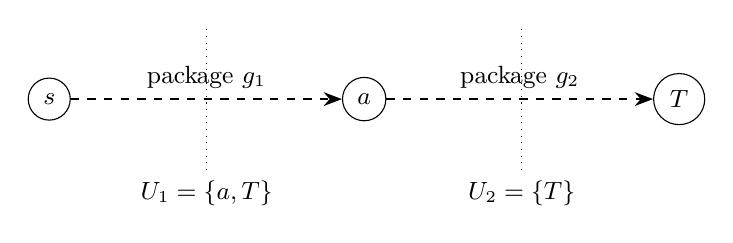
\begin{tikzpicture}[>=Stealth,every node/.style={font=\small}]
\node[draw,circle] (s) at (0,0) {$s$};
\node[draw,circle] (a) at (4,0) {$a$};
\node[draw,circle] (t) at (8,0) {$T$};
\draw[->,dashed,thick] (s)--node[above] {package $g_1$} (a);
\draw[->,dashed,thick] (a)--node[above] {package $g_2$} (t);
\draw[dotted] (2,-0.9)--(2,0.9);\draw[dotted] (6,-0.9)--(6,0.9);
\node at (2,-1.2) {$U_1=\{a,T\}$};\node at (6,-1.2) {$U_2=\{T\}$};
\end{tikzpicture}
\caption{Complementary packages. The baseline has neither edge; either package alone is insufficient, whereas both cross the two missing cuts. These are abstract packages, not automatically admissible historical GBG+S atoms.}
\end{figure}
\begin{example}[A conditional finite improvement]
Suppose the full object calculus already validates $s\to a$ and $a\to T$ but the initial operational catalogue exposes neither. Under the monotone repair hypotheses, two legal packages expose the respective existing inference instances. Their exercise plus proof execution yields a finite cost witness, whereas the baseline cannot settle. The object theory is unchanged. The example does not show that such packages exist in every GBG+S game or that either can be discovered effectively.
\end{example}

\paragraph{Why the general sovereign case is different.} Gifts may remove permissions, revise representation, require an ordered support-indexed grammar or change which later gift is admissible. Cumulative consistency, actual authorized exercise, lifecycle, unique sovereign office, provenance and all resource costs must be checked for the complete history. Set cover does not model those dependencies. The actual object-game transition system, enclosing game of admission and exercise, and target receipt must be distinguished. A full state-space construction, with version and history included, can use a settlement-game certificate instead of the monotone formula closure model. Where adversarial successors exist, a single repaired path is not a winning strategy; a forced result needs all-outcome coverage. No unrestricted syntactic relative-consistency theorem or general consistency oracle is assumed.

\paragraph{A proposed discovery cycle.} A mathematical navigator first obtains a scoped obstruction, then imagines a capability that crosses it, then tests whether the new capability is useful in a complete candidate continuation. A candidate revision is not admitted merely because it makes a lower bound smaller. It needs a typed contract and an external cumulative-consistency and preservation receipt, legal authorization and actual execution. The final proof needs the same complete-packet acceptance as before. In this sense a navigator can investigate changes to its own roads without gaining the authority to declare a theorem true.

\section{Conclusion and research obligations}
The general contribution is a deductive interpretation and certificate-oriented development of proof--obstruction duality. It connects sufficient supports, unavoidable crossings, lower-bound accounting, knowledge growth and transfer through optimistic abstractions. In a restricted finite repair model it also identifies which combinations of operational capabilities suffice to remove every baseline obstruction. None of these results requires sovereignty as a starting assumption.

The principal open problems are to find compact abstraction contracts for useful infinite rule families; determine tractable cut-price and certificate-reuse subclasses; measure the net value of obstruction-guided search against fair and heuristic comparators; and generalize the repair criterion to ordered, interacting, adversarial sovereign histories. The MAPQUEST extension is the first intended application, not a prerequisite of the mathematics.

\noindent\textbf{Evidence status.} The theorems are manuscript-level arguments under explicit assumptions. The original edition reports an executed finite test; the exact original script was not supplied for this audit. The v2 audit also independently checks the finite identities with a separate reproducible script (Section 7); neither is a proof-assistant check. The literature comparison identifies close precedents but is not exhaustive. No module has been installed, no existing publication has been modified, and no new empirical theorem-proving speedup is claimed. Research direction is attributed to Brian Tenneson; the drafting and analysis were AI-assisted. The term Picard denotes the conversational research protocol, not a claim of an independently deployed agent.

\begin{thebibliography}{99}\small
\bibitem{survey} G. Ausiello and L. Laura, ``Directed hypergraphs: Introduction and fundamental algorithms---A survey,'' \emph{Theoretical Computer Science}, 2017. \url{https://www.sciencedirect.com/science/article/pii/S0304397516002097}.
\bibitem{eiter} T. Eiter and G. Gottlob, ``Identifying the minimal transversals of a hypergraph and related problems,'' \emph{SIAM Journal on Computing}, 1995. \url{https://doi.org/10.1137/S0097539793250299}.
\bibitem{krieger} S. Krieger and J. Kececioglu, ``Computing shortest hyperpaths for pathway inference in cellular reaction networks,'' RECOMB, LNBI 13976, pp. 155--173, 2023. See the authors' algorithm description: \url{https://hyperpaths.cs.arizona.edu/}.
\bibitem{heuristic} S. Krieger and J. Kececioglu, ``Heuristic shortest hyperpaths in cell signaling hypergraphs,'' \emph{Algorithms for Molecular Biology}, 17:12, 2022. \url{https://doi.org/10.1186/s13015-022-00217-9}.
\bibitem{map1} B. Tenneson, \emph{MAPQUEST for Formal Proof: A Hilbert--Tenneson Navigation Algorithm for Verifier-Gated Automated Theorem Proving}, September 2026, ATLAS corrective edition v2, November 8, 2026. Supplied manuscript.
\bibitem{map2} B. Tenneson, \emph{MAPQUEST: Hilbert-Fair Navigation: From Addressable Inferences to a Verified Target}, September 2026, ATLAS corrective edition v2, November 8, 2026. Supplied manuscript.
\bibitem{map3} B. Tenneson, \emph{MAPQUEST III: Target Certification}, September 2026, ATLAS corrective edition v2, November 8, 2026. Supplied manuscript.
\bibitem{basin} B. Tenneson (research direction), ChatGPT (analysis), \emph{Basin Escape: Sufficient Conditions, Guarantees, and Limits}, v0.3, sovereign-game edition, November 24, 2026. Supplied manuscript.
\bibitem{cdf} B. Tenneson, with OpenAI assistance, \emph{CDF: Certified Discovery Federation}, version 13, November 23, 2026, especially Section 21. Supplied manuscript.
\end{thebibliography}
\end{document}
